\chapter{Portfolio Optimization}\label{portfolio-optimization}

Portfolio optimization models are concerned with investment where there
are typically two criteria: expected return and risk.
The investor wants
the former to be high and the latter to be low. 

There is a variety of
measures of risk. The most popular measure of risk has been variance in
return. Even though there are some problems with it, we will first look
at it very closely before introducing some alternatives.

Some notations that will be heavily used later are:

\begin{itemize}
\tightlist
\item
  expected return: \[ E(R_{p}) = \sum _{i}w_{i} E(R_{i}) \] where
  \(R_{p}\) is the return on the portfolio, \(R_{i}\) is the return on
  asset \(i\) and \(w_{i}\) is the weighting of component asset \(i\)
  (that is, the proportion of asset \(i\) in the portfolio) and
  \(\sum_{i}w_i = 1\) and \(0 \le w_i \le 1\);
\item
  portfolio return variance:
  \[ \sigma _{p}^{2} = \sum _{i}w_{i}^{2}\sigma _{i}^{2} + \sum _{i}\sum _{j\neq i}w_{i}w_{j}\sigma _{i}\sigma _{j}\rho _{ij} \]
  where \(\sigma\) is the (sample) standard deviation of the periodic
  returns on an asset, and \(\rho _{ij}\) is the correlation coefficient
  between the returns on assets \(i\) and \(j\). In a more compact way
  it can be expressed as:
  \[ \sigma _{p}^{2}=\sum _{i}\sum _{j}w_{i}w_{j}\sigma _{ij} \] where
  \(\sigma _{ij}=\sigma _{i}\sigma _{j}\rho _{ij}\) is the (sample)
  covariance of the periodic returns on the two assets, or alternatively
  denoted as \(\Sigma\), \(\sigma (i,j)\), \(cov_{ij}\) or \(cov(i,j)\).
  In matrix notation:
  \[\sigma_p^2 = \mathbf{w^T}\Sigma\mathbf{w} \]
  where $\mathbf{w} = (w_1,w_2,\ldots,w_N)$ is the vector of weights. For a very brief introduction
  to matrices see Appendix~\ref{app:matrices};
\item
  portfolio return volatility (standard deviation):
  \[ \sigma _{p}= \sqrt{\sigma _{p}^{2}}\]
\end{itemize}

\section{The Markowitz Mean/Variance Portfolio
Model}\label{the-markowitz-meanvariance-portfolio-model}

The portfolio model, introduced by Markowitz, assumes an investor has
two considerations when constructing an investment portfolio: expected
return and variance in return (i.e., risk). Variance measures the
variability in realized return around the expected return. Hence the
Markowitz model requires two major kinds of information:

\begin{itemize}
\tightlist
\item
  the estimated expected return for each candidate investment;
\item
  the covariance matrix of returns.
\end{itemize}

The covariance matrix characterizes not only the individual variability
of the return on each investment, but also how each investment's return
tends to move with other investments.

In the following example data from Quandl will be used. The following
table shows part of the sample which include for each entry a date and
the corresponding closing price of five company stocks: AAPL, AMZN, FB,
GOOG, NFLX. Figure~\ref{fig:stocks} shows the historical series of the closing price
of the five companies.

\begin{tcolorbox}[breakable, size=fbox, boxrule=1pt, pad at break*=1mm,colback=cellbackground, colframe=cellborder]
\begin{Verbatim}[commandchars=\\\{\}]
\PY{k+kn}{import} \PY{n+nn}{pandas} \PY{k}{as} \PY{n+nn}{pd}

\PY{n}{temp} \PY{o}{=} \PY{n}{pd}\PY{o}{.}\PY{n}{read\PYZus{}csv}\PY{p}{(}\PY{l+s+s2}{\PYZdq{}}\PY{l+s+s2}{quandl.csv}\PY{l+s+s2}{\PYZdq{}}\PY{p}{)}
\PY{n}{clean} \PY{o}{=} \PY{n}{temp}\PY{o}{.}\PY{n}{set\PYZus{}index}\PY{p}{(}\PY{l+s+s1}{\PYZsq{}}\PY{l+s+s1}{date}\PY{l+s+s1}{\PYZsq{}}\PY{p}{)}
\PY{n}{df} \PY{o}{=} \PY{n}{clean}\PY{o}{.}\PY{n}{pivot}\PY{p}{(}\PY{n}{columns}\PY{o}{=}\PY{l+s+s1}{\PYZsq{}}\PY{l+s+s1}{ticker}\PY{l+s+s1}{\PYZsq{}}\PY{p}{)}

\PY{n+nb}{print} \PY{p}{(}\PY{n}{df}\PY{o}{.}\PY{n}{head}\PY{p}{(}\PY{p}{)}\PY{p}{)}

            adj\_close
ticker           AAPL    AMZN      FB GOOG       NFLX
date
2014-01-02  73.523423  397.97  54.710  NaN  51.831429
2014-01-03  71.908415  396.44  54.557  NaN  51.871429
2014-01-06  72.300536  393.63  57.200  NaN  51.367143
2014-01-07  71.783135  398.03  57.920  NaN  48.500000
2014-01-08  72.238063  401.92  58.230  NaN  48.712857
\end{Verbatim}
\end{tcolorbox}

With \texttt{pandas} the main characteristics of these time series can
be easily computed (e.g.~daily returns, covariance matrix, etc...):

\begin{tcolorbox}[breakable, size=fbox, boxrule=1pt, pad at break*=1mm,colback=cellbackground, colframe=cellborder]
\begin{Verbatim}[commandchars=\\\{\}]
\PY{c+c1}{\PYZsh{} daily returns}
\PY{n}{daily\PYZus{}returns} \PY{o}{=} \PY{n}{df}\PY{o}{.}\PY{n}{pct\PYZus{}change}\PY{p}{(}\PY{p}{)}
\PY{n}{annual\PYZus{}expected} \PY{o}{=} \PY{n}{daily\PYZus{}returns}\PY{o}{.}\PY{n}{mean}\PY{p}{(}\PY{p}{)} \PY{o}{*} \PY{l+m+mi}{252}
\PY{n+nb}{print} \PY{p}{(}\PY{l+s+s2}{\PYZdq{}}\PY{l+s+s2}{Annual expected returns: }\PY{l+s+s2}{\PYZdq{}}\PY{p}{,} \PY{n}{annual\PYZus{}expected}\PY{p}{)}

\PY{c+c1}{\PYZsh{} covariance}
\PY{n}{covariance} \PY{o}{=} \PY{n}{daily\PYZus{}returns}\PY{o}{.}\PY{n}{cov}\PY{p}{(}\PY{p}{)}
\PY{n}{annual\PYZus{}covariance} \PY{o}{=} \PY{n}{covariance} \PY{o}{*} \PY{l+m+mi}{252}
\PY{n+nb}{print} \PY{p}{(}\PY{l+s+s2}{\PYZdq{}}\PY{l+s+s2}{Annual covariance: }\PY{l+s+s2}{\PYZdq{}}\PY{p}{,} \PY{n}{annual\PYZus{}covariance}\PY{p}{)}

           adj\_close
ticker          AAPL      AMZN        FB GOOG      NFLX
date
2014-01-02       NaN       NaN       NaN  NaN       NaN
2014-01-03 -0.021966 -0.003845 -0.002797  NaN  0.000772
2014-01-06  0.005453 -0.007088  0.048445  NaN -0.009722
2014-01-07 -0.007156  0.011178  0.012587  NaN -0.055817
2014-01-08  0.006338  0.009773  0.005352  NaN  0.004389
Annual expected returns:             ticker
adj\_close  AAPL      0.222314
           AMZN      0.357435
           FB        0.281059
           GOOG      0.172818
           NFLX      0.505967
dtype: float64
Annual covariance:                   adj\_close
ticker                AAPL      AMZN        FB      GOOG      NFLX
          ticker
adj\_close AAPL    0.052137  0.023737  0.024878  0.022454  0.025640
          AMZN    0.023737  0.087651  0.042694  0.039501  0.047044
          FB      0.024878  0.042694  0.078060  0.036127  0.043811
          GOOG    0.022454  0.039501  0.036127  0.051797  0.040390
          NFLX    0.025640  0.047044  0.043811  0.040390  0.180858
\end{Verbatim}
\end{tcolorbox}

\begin{figure}[htb]
\centering
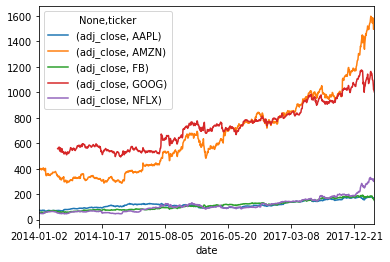
\includegraphics[width=0.7\textwidth]{figures/portfolio_sample}
\caption{Historical series of the closing price of five companies.}
\label{fig:stocks}
\end{figure}
    
The correlation matrix makes it more obvious how two random variables
move together. The correlation between two random variables equals the
covariance between the two variables, divided by the product of the
standard deviations of the two random variables. The correlation can be
between -1 and +1 with +1 (-1) being perfect correlation
(anti-correlation) between the two.

Simulating a large number of set of weights to construct portfolios with the five stocks shown before, we can see which is the
distribution of these portfolios in terms of return and volatility, see Figure~\ref{fig:mc_portfolio}.

\begin{figure}[hbt]
\centering
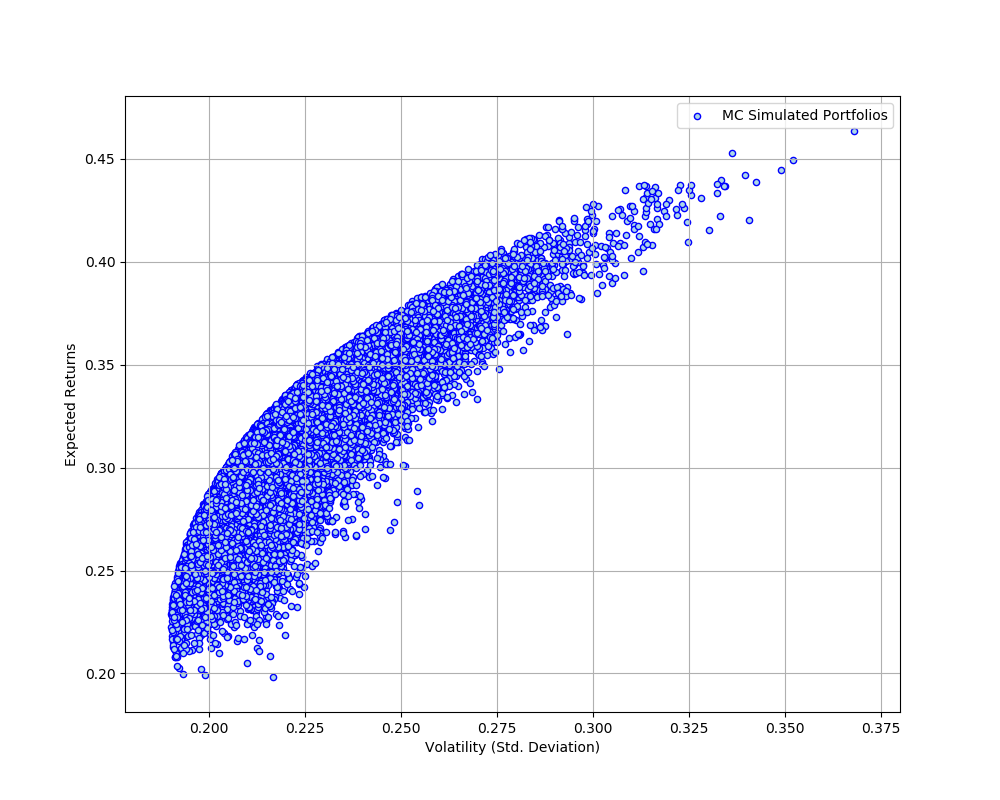
\includegraphics[width=0.8\textwidth]{figures/return_variance}
\caption{Distribution in the expected return/volatility plane of a large number of simulated portfolios.}
\label{fig:mc_portfolio}
\end{figure}


\section{Optimisation}\label{optimization}

Remembering that \(w_i\) represents the fraction of the portfolio
devoted to each stock (weights), Markowitz model states that these
weights should be chosen such that the portfolio volatility (or its
variance) is minimised. So the application of Markovitz model reduces to
an optimisation problem: given the covariance matrix of the portfolio
\(\sigma_p^2\) estimated before from the historical series, we need to find:

\[ J = \textrm{min}(\sigma_p^2) \]
with the usual constraints \(\sum_{i}w_i = 1\) and \(0 \le w_i \le 1\).

In \texttt{python} we already know how to solve a minimisation problem
(see bootstrapping in Chapter~\ref{swaps-and-bootstrapping---practical-lesson-5}) so it is enough to repeat the same steps:

\begin{itemize}
\tightlist
\item
  define an objective function (in this case the variance of the
  portfolio);
\item
  define a set of constraints (the weights constraints);
\item
  set an initial guess for the weights;
\item
  pass everything to \texttt{scipy.optimize.minimize} algorithm.
\end{itemize}

\begin{tcolorbox}[breakable, size=fbox, boxrule=1pt, pad at break*=1mm,colback=cellbackground, colframe=cellborder]
\begin{Verbatim}[commandchars=\\\{\}]
\PY{k+kn}{import} \PY{n+nn}{numpy} \PY{k}{as} \PY{n+nn}{np}\PY{o}{,} \PY{n+nn}{matplotlib}\PY{n+nn}{.}\PY{n+nn}{pyplot} \PY{k}{as} \PY{n+nn}{plt}\PY{o}{,} \PY{n+nn}{scipy}\PY{n+nn}{.}\PY{n+nn}{optimize} \PY{k}{as} \PY{n+nn}{optimize}

\PY{k}{def} \PY{n+nf}{sumWeights}\PY{p}{(}\PY{n}{weights}\PY{p}{)}\PY{p}{:}
    \PY{k}{return} \PY{n}{np}\PY{o}{.}\PY{n}{sum}\PY{p}{(}\PY{n}{weights}\PY{p}{)} \PY{o}{\PYZhy{}} \PY{l+m+mi}{1}

\PY{k}{def} \PY{n+nf}{objective}\PY{p}{(}\PY{n}{weights}\PY{p}{,} \PY{n}{covariance}\PY{p}{)}\PY{p}{:}
    \PY{k}{return} \PY{n}{np}\PY{o}{.}\PY{n}{sqrt}\PY{p}{(}\PY{n}{np}\PY{o}{.}\PY{n}{dot}\PY{p}{(}\PY{n}{weights}\PY{o}{.}\PY{n}{T}\PY{p}{,} \PY{n}{np}\PY{o}{.}\PY{n}{dot}\PY{p}{(}\PY{n}{covariance}\PY{p}{,} \PY{n}{weights}\PY{p}{)}\PY{p}{)}\PY{p}{)}

\PY{n}{numAssets} \PY{o}{=} \PY{l+m+mi}{5}
\PY{n}{constraints} \PY{o}{=} \PY{p}{(}\PY{p}{\PYZob{}}\PY{l+s+s1}{\PYZsq{}}\PY{l+s+s1}{type}\PY{l+s+s1}{\PYZsq{}}\PY{p}{:} \PY{l+s+s1}{\PYZsq{}}\PY{l+s+s1}{eq}\PY{l+s+s1}{\PYZsq{}}\PY{p}{,} \PY{l+s+s1}{\PYZsq{}}\PY{l+s+s1}{fun}\PY{l+s+s1}{\PYZsq{}}\PY{p}{:} \PY{n}{sumWeights}\PY{p}{\PYZcb{}}\PY{p}{,}\PY{p}{)}
\PY{n}{bounds} \PY{o}{=} \PY{n+nb}{tuple}\PY{p}{(}\PY{p}{(}\PY{l+m+mi}{0}\PY{p}{,} \PY{l+m+mi}{1}\PY{p}{)} \PY{k}{for} \PY{n}{asset} \PY{o+ow}{in} \PY{n+nb}{range}\PY{p}{(}\PY{n}{numAssets}\PY{p}{)}\PY{p}{)}

\PY{n}{opts} \PY{o}{=} \PY{n}{optimize}\PY{o}{.}\PY{n}{minimize}\PY{p}{(}\PY{n}{objective}\PY{p}{,} \PY{n}{np}\PY{o}{.}\PY{n}{ones}\PY{p}{(}\PY{n}{numAssets}\PY{p}{)} \PY{o}{/} \PY{n+nb}{float}\PY{p}{(}\PY{n}{numAssets}\PY{p}{)}\PY{p}{,} 
			\PY{n}{args}\PY{o}{=}\PY{p}{(}\PY{n}{annual\PYZus{}covariance}\PY{p}{,}\PY{p}{)}\PY{p}{,} 
			\PY{n}{bounds}\PY{o}{=}\PY{n}{bounds}\PY{p}{,} \PY{n}{constraints}\PY{o}{=}\PY{n}{constraints}\PY{p}{)}

\PY{n+nb}{print} \PY{p}{(}\PY{l+s+s2}{\PYZdq{}}\PY{l+s+s2}{Optimization results:}\PY{l+s+se}{\PYZbs{}n}\PY{l+s+s2}{\PYZdq{}}\PY{p}{,} \PY{n}{opts}\PY{p}{)}

\PY{n+nb}{print} \PY{p}{(}\PY{l+s+s2}{\PYZdq{}}\PY{l+s+se}{\PYZbs{}n}\PY{l+s+s2}{Recommended weights: }\PY{l+s+s2}{\PYZdq{}}\PY{p}{,} \PY{n}{opts}\PY{o}{.}\PY{n}{x}\PY{p}{)}
\PY{n+nb}{print} \PY{p}{(}\PY{l+s+s2}{\PYZdq{}}\PY{l+s+s2}{Portfolio expected annual return: }\PY{l+s+si}{\PYZob{}:.4f\PYZcb{}}\PY{l+s+s2}{\PYZdq{}}\PY{o}{.}\PY{n}{format}
				\PY{p}{(}\PY{n}{np}\PY{o}{.}\PY{n}{sum}\PY{p}{(}\PY{n}{annual\PYZus{}expected}\PY{o}{*}\PY{n}{opts}\PY{o}{.}\PY{n}{x}\PY{p}{)}\PY{p}{)}\PY{p}{)}

Optimization results:
      fun: 0.18996519187658553
     jac: array([0.19007478, 0.19040664, 0.18950935, 0.1898793 , 0.18995349])
 message: 'Optimization terminated successfully.'
    nfev: 63
     nit: 9
    njev: 9
  status: 0
 success: True
       x: array([0.44735955, 0.06873074, 0.10429827, 0.36908076, 0.01053068])

Recommended weights:  [0.44735955 0.06873074 0.10429827 0.36908076 0.01053068]
Portfolio expected annual return: 0.2224
    \end{Verbatim}
\end{tcolorbox}

The solution recommends about 44\% of the portfolio be invested in AAPL,
about 7\% in AMZN, 10\% in FB and so on\ldots{} The expected return is
about 22\%, with a variance of about 0.036 or, equivalently, a standard deviation of 0.19.

In this example we based the model simply on straightforward statistical
data derived from daily returns. However it could be possible, rather
than use historical data for estimating the expected return of an asset,
to base this estimate on more current, proprietary information about
expected future performance of the asset.

\section{Efficient Frontier}\label{efficient-frontier}

There is no precise way for an investor to determine the ``correct''
working point between risk and return. For example if an investor wants
a higher expected return, she generally has to ``pay for it'' with
higher risk. Thus, one is frequently interested in looking at the
distribution of the trade off between the two. In finance terminology, we
would like to trace out the \emph{efficient frontier} of return and
risk. This is doable solving for the minimum variance portfolio over a
range of values for the expected return (e.g.~ranging from 0.20 to
0.45).
Now in the code, beside the usual constraint on the sum of the weights, we have to add the one that force the resulting return to be equal to the chosen target.

The following code produce the efficient frontier plot shown in Fig.~\ref{fig:efficient_frontier}.

\begin{tcolorbox}[breakable, size=fbox, boxrule=1pt, pad at break*=1mm,colback=cellbackground, colframe=cellborder]
\begin{Verbatim}[commandchars=\\\{\}]
\PY{k}{def} \PY{n+nf}{getTargetReturn}\PY{p}{(}\PY{n}{weights}\PY{p}{,} \PY{n}{returns}\PY{p}{,} \PY{n}{targetReturn}\PY{p}{)}\PY{p}{:}
    \PY{n}{portfolio\PYZus{}return} \PY{o}{=} \PY{n}{np}\PY{o}{.}\PY{n}{sum}\PY{p}{(}\PY{n}{returns}\PY{o}{*}\PY{n}{weights}\PY{p}{)}
    \PY{k}{return} \PY{p}{(}\PY{n}{portfolio\PYZus{}return} \PY{o}{\PYZhy{}} \PY{n}{targetReturn}\PY{p}{)}

\PY{n}{returns} \PY{o}{=} \PY{p}{[}\PY{p}{]}
\PY{k}{for} \PY{n}{eff} \PY{o+ow}{in} \PY{n}{np}\PY{o}{.}\PY{n}{arange}\PY{p}{(}\PY{l+m+mf}{0.20}\PY{p}{,} \PY{l+m+mf}{0.45}\PY{p}{,} \PY{l+m+mf}{0.005}\PY{p}{)}\PY{p}{:}
    \PY{n}{constraints} \PY{o}{=} \PY{p}{(}\PY{p}{\PYZob{}}\PY{l+s+s1}{\PYZsq{}}\PY{l+s+s1}{type}\PY{l+s+s1}{\PYZsq{}}\PY{p}{:} \PY{l+s+s1}{\PYZsq{}}\PY{l+s+s1}{eq}\PY{l+s+s1}{\PYZsq{}}\PY{p}{,} \PY{l+s+s1}{\PYZsq{}}\PY{l+s+s1}{fun}\PY{l+s+s1}{\PYZsq{}}\PY{p}{:} \PY{n}{getTargetReturn}\PY{p}{,}
                    \PY{l+s+s2}{\PYZsq{}}\PY{l+s+s2}{args}\PY{l+s+s2}{\PYZsq{}}\PY{p}{:}\PY{p}{(}\PY{n}{annual\PYZus{}expected}\PY{p}{,} \PY{n}{eff}\PY{p}{,}\PY{p}{)}\PY{p}{\PYZcb{}}\PY{p}{,}
                   \PY{p}{\PYZob{}}\PY{l+s+s1}{\PYZsq{}}\PY{l+s+s1}{type}\PY{l+s+s1}{\PYZsq{}}\PY{p}{:} \PY{l+s+s1}{\PYZsq{}}\PY{l+s+s1}{eq}\PY{l+s+s1}{\PYZsq{}}\PY{p}{,} \PY{l+s+s1}{\PYZsq{}}\PY{l+s+s1}{fun}\PY{l+s+s1}{\PYZsq{}}\PY{p}{:} \PY{n}{sumWeights}\PY{p}{\PYZcb{}}\PY{p}{)}
    \PY{n}{bounds} \PY{o}{=} \PY{n+nb}{tuple}\PY{p}{(}\PY{p}{(}\PY{l+m+mi}{0}\PY{p}{,} \PY{l+m+mi}{1}\PY{p}{)} \PY{k}{for} \PY{n}{asset} \PY{o+ow}{in} \PY{n+nb}{range}\PY{p}{(}\PY{n}{numAssets}\PY{p}{)}\PY{p}{)}
    \PY{n}{opts} \PY{o}{=} \PY{n}{optimize}\PY{o}{.}\PY{n}{minimize}\PY{p}{(}\PY{n}{objective}\PY{p}{,} \PY{n}{np}\PY{o}{.}\PY{n}{ones}\PY{p}{(}\PY{n}{numAssets}\PY{p}{)} \PY{o}{/} \PY{n+nb}{float}\PY{p}{(}\PY{n}{numAssets}\PY{p}{)}\PY{p}{,} 
                             \PY{n}{args}\PY{o}{=}\PY{p}{(}\PY{n}{annual\PYZus{}covariance}\PY{p}{,}\PY{p}{)}\PY{p}{,}
                             \PY{n}{bounds}\PY{o}{=}\PY{n}{bounds}\PY{p}{,} \PY{n}{constraints}\PY{o}{=}\PY{n}{constraints}\PY{p}{)}

    \PY{n}{returns}\PY{o}{.}\PY{n}{append}\PY{p}{(}\PY{p}{(}\PY{n}{np}\PY{o}{.}\PY{n}{sqrt}\PY{p}{(}\PY{n}{np}\PY{o}{.}\PY{n}{dot}\PY{p}{(}\PY{n}{opts}\PY{o}{.}\PY{n}{x}\PY{o}{.}\PY{n}{T}\PY{p}{,} \PY{n}{np}\PY{o}{.}\PY{n}{dot}\PY{p}{(}\PY{n}{annual\PYZus{}covariance}\PY{p}{,} \PY{n}{opts}\PY{o}{.}\PY{n}{x}\PY{p}{)}\PY{p}{)}\PY{p}{)}\PY{p}{,}
                   \PY{n}{np}\PY{o}{.}\PY{n}{sum}\PY{p}{(}\PY{n}{annual\PYZus{}expected}\PY{o}{*}\PY{n}{opts}\PY{o}{.}\PY{n}{x}\PY{p}{)}\PY{p}{)}\PY{p}{)}

\PY{n}{returns} \PY{o}{=} \PY{n}{np}\PY{o}{.}\PY{n}{array}\PY{p}{(}\PY{n}{returns}\PY{p}{)}
\end{Verbatim}
\end{tcolorbox}

\begin{figure}[htb]
\centering
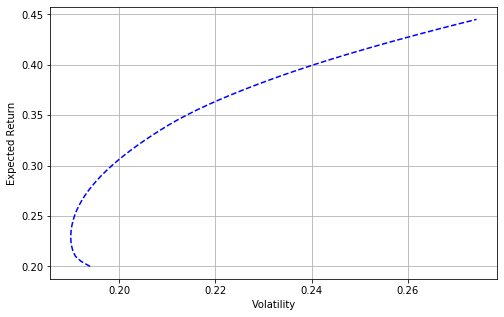
\includegraphics[width=0.7\textwidth]{figures/efficient_frontier.png}
\caption{Efficient frontier for our example portfolio obtained minimizing the the variance and requiring an expected return between 0.02 and 0.45.}
\label{fig:efficient_frontier}
\end{figure}
    
\section{Portfolios with a Risk-Free
Asset}\label{portfolios-with-a-risk-free-asset}

When one of the investments available is risk free, then the efficient
frontier has a particularly simple form, a line called the capital
allocation line (CAL). The slope of the CAL measures the trade-off
between risk and return. A higher slope means that investors receive a
higher expected return in exchange for taking on more risk. The value of
this calculation is known as the Sharpe ratio.

The capital allocation line aids investors in choosing how much to
invest in a risk-free asset and one or more risky assets.

The simplest example is a portfolio containing two assets: a risk-free
Treasury bill and a stock. Assume that the expected return of the
Treasury bill is \(\mathbb{E}(R_f)=3\%\) and its risk is 0\%. Further, assume that
the expected return of the stock is \(\mathbb{E}(R_r)=10\%\) and its standard
deviation is \(\sigma_r=20\%\). The question that needs to be answered
for any individual investor is how much to invest in each of these
assets.

The expected return (\(\mathbb{E}(R_p)\)) of this portfolio is calculated as
follows:

\[ \mathbb{E}(R_p) = \mathbb{E}(R_f)\cdot w_f + \mathbb{E}(R_r)\cdot (1- w_f) \]

where \(w_f\) is the relative allocation to the risk-free asset.

The calculation of risk for this portfolio is simple because the
standard deviation of the Treasury bill is 0\%. Thus, risk is calculated
as:

\[ \sigma_p = (1-w_f)\cdot \sigma_r \]

In this very simple example, if an investor were to invest 100\% into
the risk-free asset (\(w_f=1\)), the expected return would be 3\% and
the risk of the portfolio would be 0\%. Likewise, investing 100\% into
the stock (\(w_f=0\)) would give an investor an expected return of 10\%
and a portfolio risk of 20\%. If the investor allocated 25\% to the
risk-free asset and 75\% to the risky asset, the portfolio expected
return and risk calculations would be:

\[ \mathbb{E}(R_p) = (3\% \cdot 25\%) + (10\% \cdot 75\%) = 0.75\% + 7.5\% = 8.25\% \]

\[ \sigma_p = 75\% \cdot 20\% = 15\% \]

Applying the same reasoning to our example we can consider an additional
risk-free asset with an expected return of 10\% and repeat the
minimisation to determine the efficient frontier of the resulting
portfolio. Notice how the objective function is still the same, while
the target return constraint now includes the risk-free asset.

\begin{tcolorbox}[breakable, size=fbox, boxrule=1pt, pad at break*=1mm,colback=cellbackground, colframe=cellborder]
\begin{Verbatim}[commandchars=\\\{\}]
\PY{n}{numAssets} \PY{o}{=} \PY{l+m+mi}{6}

\PY{k}{def} \PY{n+nf}{sumWeights2}\PY{p}{(}\PY{n}{weights}\PY{p}{)}\PY{p}{:}
    \PY{k}{return} \PY{n}{np}\PY{o}{.}\PY{n}{sum}\PY{p}{(}\PY{n}{weights}\PY{p}{)} \PY{o}{\PYZhy{}} \PY{l+m+mi}{1}

\PY{k}{def} \PY{n+nf}{objective4}\PY{p}{(}\PY{n}{weights}\PY{p}{,} \PY{n}{covariance}\PY{p}{)}\PY{p}{:}
    \PY{k}{return} \PY{n}{np}\PY{o}{.}\PY{n}{sqrt}\PY{p}{(}\PY{n}{np}\PY{o}{.}\PY{n}{dot}\PY{p}{(}\PY{n}{weights}\PY{p}{[}\PY{p}{:}\PY{o}{\PYZhy{}}\PY{l+m+mi}{1}\PY{p}{]}\PY{o}{.}\PY{n}{T}\PY{p}{,} \PY{n}{np}\PY{o}{.}\PY{n}{dot}\PY{p}{(}\PY{n}{covariance}\PY{p}{,} \PY{n}{weights}\PY{p}{[}\PY{p}{:}\PY{o}{\PYZhy{}}\PY{l+m+mi}{1}\PY{p}{]}\PY{p}{)}\PY{p}{)}\PY{p}{)}

\PY{k}{def} \PY{n+nf}{getTargetReturn2}\PY{p}{(}\PY{n}{weights}\PY{p}{,} \PY{n}{returns}\PY{p}{,} \PY{n}{targetReturn}\PY{p}{,} \PY{n}{risk\PYZus{}free}\PY{p}{)}\PY{p}{:}
    \PY{n}{portfolio\PYZus{}return} \PY{o}{=} \PY{n}{np}\PY{o}{.}\PY{n}{sum}\PY{p}{(}\PY{n}{returns}\PY{o}{*}\PY{n}{weights}\PY{p}{[}\PY{p}{:}\PY{o}{\PYZhy{}}\PY{l+m+mi}{1}\PY{p}{]}\PY{p}{)} \PY{o}{+} \PY{p}{(}\PY{n}{weights}\PY{p}{[}\PY{l+m+mi}{5}\PY{p}{]}\PY{p}{)} \PY{o}{*} \PY{n}{risk\PYZus{}free}
    \PY{k}{return} \PY{p}{(}\PY{n}{portfolio\PYZus{}return} \PY{o}{\PYZhy{}} \PY{n}{targetReturn}\PY{p}{)}

\PY{n}{rfAssetReturn} \PY{o}{=} \PY{l+m+mf}{0.10}
\PY{n}{returns2} \PY{o}{=} \PY{p}{[}\PY{p}{]}
\PY{k}{for} \PY{n}{eff} \PY{o+ow}{in} \PY{n}{np}\PY{o}{.}\PY{n}{arange}\PY{p}{(}\PY{l+m+mf}{0.10}\PY{p}{,} \PY{l+m+mf}{0.40}\PY{p}{,} \PY{l+m+mf}{0.01}\PY{p}{)}\PY{p}{:}
    \PY{n}{constraints} \PY{o}{=} \PY{p}{(}\PY{p}{\PYZob{}}\PY{l+s+s1}{\PYZsq{}}\PY{l+s+s1}{type}\PY{l+s+s1}{\PYZsq{}}\PY{p}{:} \PY{l+s+s1}{\PYZsq{}}\PY{l+s+s1}{eq}\PY{l+s+s1}{\PYZsq{}}\PY{p}{,} \PY{l+s+s1}{\PYZsq{}}\PY{l+s+s1}{fun}\PY{l+s+s1}{\PYZsq{}}\PY{p}{:} \PY{n}{getTargetReturn2}\PY{p}{,} 
    		  \PY{l+s+s2}{\PYZdq{}}\PY{l+s+s2}{args}\PY{l+s+s2}{\PYZdq{}}\PY{p}{:}\PY{p}{(}\PY{n}{annual\PYZus{}expected}\PY{p}{,} \PY{n}{eff}\PY{p}{,} \PY{n}{rfAssetReturn}\PY{p}{)}\PY{p}{\PYZcb{}}\PY{p}{,}
                   \PY{p}{\PYZob{}}\PY{l+s+s1}{\PYZsq{}}\PY{l+s+s1}{type}\PY{l+s+s1}{\PYZsq{}}\PY{p}{:} \PY{l+s+s1}{\PYZsq{}}\PY{l+s+s1}{eq}\PY{l+s+s1}{\PYZsq{}}\PY{p}{,} \PY{l+s+s1}{\PYZsq{}}\PY{l+s+s1}{fun}\PY{l+s+s1}{\PYZsq{}}\PY{p}{:} \PY{n}{sumWeights2}\PY{p}{\PYZcb{}}\PY{p}{)}
    \PY{n}{bounds} \PY{o}{=} \PY{n+nb}{tuple}\PY{p}{(}\PY{p}{(}\PY{l+m+mi}{0}\PY{p}{,} \PY{l+m+mi}{1}\PY{p}{)} \PY{k}{for} \PY{n}{asset} \PY{o+ow}{in} \PY{n+nb}{range}\PY{p}{(}\PY{n}{numAssets}\PY{p}{)}\PY{p}{)}
    \PY{n}{opts} \PY{o}{=} \PY{n}{optimize}\PY{o}{.}\PY{n}{minimize}\PY{p}{(}\PY{n}{objective4}\PY{p}{,} \PY{n}{np}\PY{o}{.}\PY{n}{ones}\PY{p}{(}\PY{n}{numAssets}\PY{p}{)} \PY{o}{/} \PY{n+nb}{float}\PY{p}{(}\PY{n}{numAssets}\PY{p}{)}\PY{p}{,} 
    			    \PY{n}{args}\PY{o}{=}\PY{p}{(}\PY{n}{annual\PYZus{}covariance}\PY{p}{)}\PY{p}{,}
                             \PY{n}{bounds}\PY{o}{=}\PY{n}{bounds}\PY{p}{,} \PY{n}{constraints}\PY{o}{=}\PY{n}{constraints}\PY{p}{)}
    \PY{k}{if} \PY{n}{eff} \PY{o}{\PYZgt{}}\PY{o}{=} \PY{l+m+mf}{0.3}\PY{p}{:}
        \PY{n+nb}{print} \PY{p}{(}\PY{n}{opts}\PY{o}{.}\PY{n}{x}\PY{p}{)}

    \PY{n}{returns2}\PY{o}{.}\PY{n}{append}\PY{p}{(}\PY{p}{(}\PY{n}{np}\PY{o}{.}\PY{n}{sqrt}\PY{p}{(}\PY{n}{np}\PY{o}{.}\PY{n}{dot}\PY{p}{(}\PY{n}{opts}\PY{o}{.}\PY{n}{x}\PY{p}{[}\PY{p}{:}\PY{o}{\PYZhy{}}\PY{l+m+mi}{1}\PY{p}{]}\PY{o}{.}\PY{n}{T}\PY{p}{,} \PY{n}{np}\PY{o}{.}\PY{n}{dot}\PY{p}{(}\PY{n}{annual\PYZus{}covariance}\PY{p}{,} \PY{n}{opts}\PY{o}{.}\PY{n}{x}\PY{p}{[}\PY{p}{:}\PY{o}{\PYZhy{}}\PY{l+m+mi}{1}\PY{p}{]}\PY{p}{)}\PY{p}{)}\PY{p}{)}\PY{p}{,} 
                    
\PY{n}{np}\PY{o}{.}\PY{n}{sum}\PY{p}{(}\PY{n}{annual\PYZus{}expected}\PY{o}{*}\PY{n}{opts}\PY{o}{.}\PY{n}{x}\PY{p}{[}\PY{p}{:}\PY{o}{\PYZhy{}}\PY{l+m+mi}{1}\PY{p}{]}\PY{p}{)}\PY{o}{+}\PY{n}{opts}\PY{o}{.}\PY{n}{x}\PY{p}{[}\PY{l+m+mi}{5}\PY{p}{]}\PY{o}{*}\PY{n}{rfAssetReturn}\PY{p}{)}\PY{p}{)}
\PY{n}{returns2} \PY{o}{=} \PY{n}{np}\PY{o}{.}\PY{n}{array}\PY{p}{(}\PY{n}{returns2}\PY{p}{)}
\end{Verbatim}
\end{tcolorbox}

\begin{figure}[htb]
\centering
    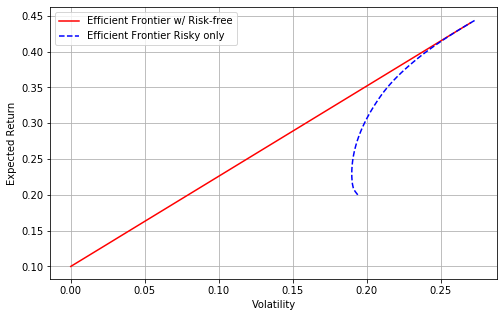
\includegraphics[width=0.7\textwidth]{figures/cal.png}
    \caption{Comparison of efficient frontier with a risk-free asset (red) and with risky asset only (blue).}
    \label{fig:cal}
\end{figure}
    
As it is clear from Fig.~\ref{fig:cal} the efficient frontier has become a
straight line, tangent to the frontier of the risky assets only. When
the target is 10\% the entire investment is allocated to the risk-free
asset, as the target increases the fraction of the risky assets grows
proportionally to the volatility. 

It is important to notice that in general the relative proportions
devoted to risky investments do not change. Only the allocation between
the risk-free asset and the risky assets change.

\subsection{The Sharpe Ratio}\label{the-sharpe-ratio}

For some portfolio \(p\), of risky assets, excluding the risk-free
asset, let it be:

\begin{itemize}
\tightlist
\item
  \(R_p\) its expected return;
\item
  \(\sigma_p\) its standard deviation in return;
\item
  \(r_0\) the return of the risk-free asset.
\end{itemize}

A plausible single measure (as opposed to the two measures, risk and
return) of attractiveness of portfolio \(p\) is the Sharpe ratio:

\[ \cfrac{R_p - r_0}{\sigma_p} \]

In words, it measures how much additional return we achieved for the
additional risk we took on, relative to putting all our money in the
risk-free asset. The portfolio that maximizes this ratio has a certain
well-defined appeal. Suppose:

\begin{itemize}
\tightlist
\item
  \(t\) our desired target return;
\item
  \(w_p\) the fraction of our wealth we place in portfolio \(p\) (the
  rest placed in the risk-free asset).
\end{itemize}

To meet our return target, we must have:

\[ (1 - w_p) * r_0 + w_p * R_p = t \]

The standard deviation of our total investment is:
\(w_p\cdot \sigma_p\). Solving for \(w_p\) in the equation above, we
get:

\[ w_p = \cfrac{t - r_0}{R_p - r_0} \]

Thus, the standard deviation of the portfolio is:

\[ w_p\cdot \sigma_p = \Big[\cfrac{t - r_0}{R_p - r_0}\Big]\cdot \sigma_p \]

Minimising the portfolio standard deviation means:

\[ \textrm{min}\Big(\Big[\cfrac{t - r_0}{R_p - r_0}\Big]\cdot \sigma_p\Big)\implies\textrm{max}\Big(\cfrac{R_p - r_0}{\sigma_p}\Big) \]

So, regardless of our risk/return preference, the money we invest in
risky assets should be invested in the risky portfolio that maximises
the Sharpe ratio.

Let's see the application of the Sharpe ration on our sample:

\begin{tcolorbox}[breakable, size=fbox, boxrule=1pt, pad at break*=1mm,colback=cellbackground, colframe=cellborder]
\begin{Verbatim}[commandchars=\\\{\}]
\PY{n}{numAssets} \PY{o}{=} \PY{l+m+mi}{5}
\PY{n}{riskFreeRate} \PY{o}{=} \PY{l+m+mf}{0.10}
\PY{n}{args} \PY{o}{=} \PY{p}{(}\PY{n}{annual\PYZus{}expected}\PY{p}{,} \PY{n}{riskFreeRate}\PY{p}{,} \PY{n}{annual\PYZus{}covariance}\PY{p}{)}

\PY{k}{def} \PY{n+nf}{negativeSharpeRatio}\PY{p}{(}\PY{n}{weights}\PY{p}{,} \PY{n}{annualReturns}\PY{p}{,} \PY{n}{riskFreeRate}\PY{p}{,} \PY{n}{annual\PYZus{}covariance}\PY{p}{)}\PY{p}{:}
    \PY{n}{p\PYZus{}ret} \PY{o}{=} \PY{n}{np}\PY{o}{.}\PY{n}{sum}\PY{p}{(}\PY{n}{annualReturns}\PY{o}{*}\PY{n}{weights}\PY{p}{)}
    \PY{n}{p\PYZus{}var} \PY{o}{=} \PY{n}{np}\PY{o}{.}\PY{n}{sqrt}\PY{p}{(}\PY{n}{np}\PY{o}{.}\PY{n}{dot}\PY{p}{(}\PY{n}{weights}\PY{o}{.}\PY{n}{T}\PY{p}{,} \PY{n}{np}\PY{o}{.}\PY{n}{dot}\PY{p}{(}\PY{n}{annual\PYZus{}covariance}\PY{p}{,} \PY{n}{weights}\PY{p}{)}\PY{p}{)}\PY{p}{)}
    \PY{n}{ratio} \PY{o}{=} \PY{o}{\PYZhy{}}\PY{p}{(}\PY{n}{p\PYZus{}ret} \PY{o}{\PYZhy{}} \PY{n}{riskFreeRate}\PY{p}{)} \PY{o}{/} \PY{n}{p\PYZus{}var}
    \PY{k}{return} \PY{n}{ratio}
    
\PY{n}{constraints} \PY{o}{=} \PY{p}{(}\PY{p}{\PYZob{}}\PY{l+s+s1}{\PYZsq{}}\PY{l+s+s1}{type}\PY{l+s+s1}{\PYZsq{}}\PY{p}{:} \PY{l+s+s1}{\PYZsq{}}\PY{l+s+s1}{eq}\PY{l+s+s1}{\PYZsq{}}\PY{p}{,} \PY{l+s+s1}{\PYZsq{}}\PY{l+s+s1}{fun}\PY{l+s+s1}{\PYZsq{}}\PY{p}{:} \PY{n}{sumWeights}\PY{p}{\PYZcb{}}\PY{p}{)}
\PY{n}{bounds} \PY{o}{=} \PY{n+nb}{tuple}\PY{p}{(}\PY{p}{(}\PY{l+m+mi}{0}\PY{p}{,} \PY{l+m+mi}{1}\PY{p}{)} \PY{k}{for} \PY{n}{asset} \PY{o+ow}{in} \PY{n+nb}{range}\PY{p}{(}\PY{n}{numAssets}\PY{p}{)}\PY{p}{)}

\PY{n}{opts} \PY{o}{=} \PY{n}{optimize}\PY{o}{.}\PY{n}{minimize}\PY{p}{(}\PY{n}{negativeSharpeRatio}\PY{p}{,} \PY{n}{np}\PY{o}{.}\PY{n}{ones}\PY{p}{(}\PY{n}{numAssets}\PY{p}{)} \PY{o}{/} \PY{n+nb}{float}\PY{p}{(}\PY{n}{numAssets}\PY{p}{)}\PY{p}{,} \PY{n}{args}\PY{o}{=}\PY{n}{args}\PY{p}{,}
                         \PY{n}{bounds}\PY{o}{=}\PY{n}{bounds}\PY{p}{,} \PY{n}{constraints}\PY{o}{=}\PY{n}{constraints}\PY{p}{)}

\PY{n+nb}{print} \PY{p}{(}\PY{l+s+s2}{\PYZdq{}}\PY{l+s+s2}{Optimized weights: }\PY{l+s+s2}{\PYZdq{}}\PY{p}{,} \PY{n}{opts}\PY{o}{.}\PY{n}{x}\PY{p}{)}

\PY{n}{ret} \PY{o}{=} \PY{n}{np}\PY{o}{.}\PY{n}{sum}\PY{p}{(}\PY{n}{annual\PYZus{}expected}\PY{o}{*}\PY{n}{opts}\PY{o}{.}\PY{n}{x}\PY{p}{)}
\PY{n}{vol} \PY{o}{=} \PY{n}{np}\PY{o}{.}\PY{n}{sqrt}\PY{p}{(}\PY{n}{np}\PY{o}{.}\PY{n}{dot}\PY{p}{(}\PY{n}{opts}\PY{o}{.}\PY{n}{x}\PY{o}{.}\PY{n}{T}\PY{p}{,} \PY{n}{np}\PY{o}{.}\PY{n}{dot}\PY{p}{(}\PY{n}{annual\PYZus{}covariance}\PY{p}{,} \PY{n}{opts}\PY{o}{.}\PY{n}{x}\PY{p}{)}\PY{p}{)}\PY{p}{)}

\PY{n+nb}{print} \PY{p}{(}\PY{l+s+s2}{\PYZdq{}}\PY{l+s+s2}{Sharpe ratio: }\PY{l+s+s2}{\PYZdq{}}\PY{p}{,} \PY{o}{\PYZhy{}}\PY{n}{opts}\PY{o}{.}\PY{n}{fun}\PY{p}{)}

\PY{n}{plt}\PY{o}{.}\PY{n}{plot}\PY{p}{(}\PY{n}{returns}\PY{p}{[}\PY{p}{:}\PY{p}{,}\PY{l+m+mi}{0}\PY{p}{]}\PY{p}{,} \PY{n}{returns}\PY{p}{[}\PY{p}{:}\PY{p}{,}\PY{l+m+mi}{1}\PY{p}{]}\PY{p}{,} \PY{n}{label}\PY{o}{=}\PY{l+s+s2}{\PYZdq{}}\PY{l+s+s2}{Efficient Frontier w/o risk\PYZhy{}free asset}\PY{l+s+s2}{\PYZdq{}}\PY{p}{)}
\PY{n}{plt}\PY{o}{.}\PY{n}{plot}\PY{p}{(}\PY{n}{returns2}\PY{p}{[}\PY{p}{:}\PY{p}{,}\PY{l+m+mi}{0}\PY{p}{]}\PY{p}{,} \PY{n}{returns2}\PY{p}{[}\PY{p}{:}\PY{p}{,}\PY{l+m+mi}{1}\PY{p}{]}\PY{p}{,} \PY{n}{label}\PY{o}{=}\PY{l+s+s2}{\PYZdq{}}\PY{l+s+s2}{Efficient Frontier w/ risk\PYZhy{}free asset}\PY{l+s+s2}{\PYZdq{}}\PY{p}{)}
\PY{n}{plt}\PY{o}{.}\PY{n}{xlabel}\PY{p}{(}\PY{l+s+s2}{\PYZdq{}}\PY{l+s+s2}{Volatility}\PY{l+s+s2}{\PYZdq{}}\PY{p}{)}
\PY{n}{plt}\PY{o}{.}\PY{n}{ylabel}\PY{p}{(}\PY{l+s+s2}{\PYZdq{}}\PY{l+s+s2}{Expected Return}\PY{l+s+s2}{\PYZdq{}}\PY{p}{)}
\PY{n}{plt}\PY{o}{.}\PY{n}{scatter}\PY{p}{(}\PY{n}{vol}\PY{p}{,} \PY{n}{ret}\PY{p}{,} \PY{n}{label}\PY{o}{=}\PY{l+s+s2}{\PYZdq{}}\PY{l+s+s2}{Sharpe Portfolio}\PY{l+s+s2}{\PYZdq{}}\PY{p}{)}
\PY{n}{plt}\PY{o}{.}\PY{n}{legend}\PY{p}{(}\PY{p}{)}
\PY{n}{plt}\PY{o}{.}\PY{n}{show}\PY{p}{(}\PY{p}{)}
\PY{n}{a} \PY{o}{=} \PY{p}{[}\PY{l+m+mf}{1.06162709e\PYZhy{}01}\PY{p}{,} \PY{l+m+mf}{3.00245096e\PYZhy{}01}\PY{p}{,} \PY{l+m+mf}{3.91027233e\PYZhy{}02}\PY{p}{,} \PY{l+m+mf}{1.86970665e\PYZhy{}16}\PY{p}{,} \PY{l+m+mf}{2.77464263e\PYZhy{}01}\PY{p}{]}
\PY{k}{for} \PY{n}{i} \PY{o+ow}{in} \PY{n}{a}\PY{p}{:}
    \PY{n+nb}{print} \PY{p}{(}\PY{n}{i}\PY{o}{/}\PY{n+nb}{sum}\PY{p}{(}\PY{n}{a}\PY{p}{)}\PY{p}{)}

Optimized weights:  [0.14534034 0.41720748 0.0539508  0.         0.38350138]
Sharpe ratio:  1.1137235916752375
\end{Verbatim}
\end{tcolorbox}

\begin{figure}[htb]
\centering
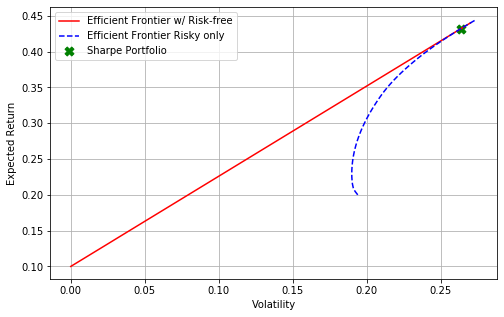
\includegraphics[width=0.7\textwidth]{figures/sharpe_ratio.png}
   \caption{Sharpe portfolio (green cross) compared to the efficient frontier with a risk-free asset (red) and with risky asset only (blue).}
\label{fig:sharpe_ratio}
\end{figure}
    
Notice that in general the relative proportions of the stocks are the
same as in the previous case where we explicitly included a risk free
asset (0.143, 0.416, 0.0532, 0., 0.383).

So the optimization using the Sharpe ratio gives us a portfolio that is
on the minimum volatility efficient frontier, and gives the maximum
return relative to putting all our money in the risk-free asset.

What is considered a good Sharpe ratio that indicates a high degree of
expected return for a relatively low amount of risk? Usually, any Sharpe
ratio greater than 1.0 is considered acceptable to good by investors. A
ratio higher than 2.0 is rated as very good. A ratio of 3.0 or higher is
considered excellent. A ratio under 1.0 is considered sub-optimal.

Figure~\ref{fig:sharpe_ratio} shows the result of the optimization for our example.

\subsection{Limits of the Markowitz
Model}\label{limits-of-the-markowitz-model}

Despite the significant utility of the Markowitz theory, there are some
major limitations in this model:

\begin{itemize}
\tightlist
\item
  it is difficult to forecast asset returns with accuracy using
  historical data, which tends to be a poor forecasting source. As
  return estimations have a much larger impact on the asset allocations,
  small changes in return assumptions can lead to inefficient
  portfolios. Therefore, the model tends to lead to highly concentrated
  portfolios (out-of sample weights) that do not offer as much
  diversification benefits in practice as they seem to provide in
  theory;
\item
  the model assumes that asset correlations are linear. In reality,
  asset correlations move dynamically, changing with the market cycles.
  During the global financial crisis, asset correlations approached
  almost 1, so if anything, diversification seemed to have insignificant
  impacts on the portfolios;
\item
  last but not the least, the model assumes normality in return
  distributions. Therefore, it does not factor in extreme market moves
  which tend to make returns distributions either skewed, fat tailed or
  both. Without optimising the portfolio for asset that may actually
  have skewed distributions or fat tailed, it could lead to a riskier
  allocation that is intended.
\end{itemize}

\section{Risk Parity Portfolio}\label{risk-parity-portfolio}

An alternative approach to Markowitz theory is given by the
\emph{risk parity}. A risk parity portfolio is an investment allocation
strategy which focuses on the allocation of risk, rather than the
allocation of capital. A risk parity (equal risk) portfolio is
characterised by having equal risk contributions to the total risk from
each individual asset. For example, a typical 40\% bond 60\% equity
portfolio has a significant risk in equity, allocation according to the
risk parity principle would lead to same risk contribution between
equity and bond.

Risk parity allocation is also referred to as equally-weighted risk
contributions portfolio method. Equally-weighted risk contributions is
not about \emph{having the same volatility}, it is about having each
asset contributing in the same way to the portfolio overall volatility.
For this we will have to define the contribution of each asset to the
portfolio risk. This allocation strategy has gained popularity in the
last decades since it is believed to provide better risk adjusted return
than capital based allocation strategies.

Let's go over a very basic example to better illustrate how to construct
a simple risk parity (equal risk) portfolio. Later we will see how easy
is to extend this technique to a risk budgeting portfolio (targeted risk
allocation).

Consider a portfolio of \(N\) assets: \(x_{1}, \ldots, x_N\) where as
usual the weight of the asset \(x_{i}\) is denoted by \(w_{i}\). The
\(w_{i}\) form the allocation vector \(\mathbf{w}\). Let us further
denote the covariance matrix of the assets as \(\Sigma\). The volatility
of the portfolio is then defined as:

\[ \sigma_p={\sqrt {\mathbf{w^T}\Sigma \mathbf{w}}} = \sum _{i=1}^{N}\sigma _{i}\qquad\textrm{with}~\sigma _{i} = w_{i}\cdot \cfrac{\partial\sigma_p}{\partial w_{i}}={\cfrac {w_{i}(\Sigma \mathbf{w})_{i}}{\sqrt {\mathbf{w^T}\Sigma \mathbf{w}}}}\]
so that \(\sigma _{i}\) can be interpreted as the contribution of asset
\(i\) in the portfolio to the overall risk of the portfolio.
Equal risk contribution then means \(\sigma _{i} =\sigma _{j}\) for all
\(i,j\) or equivalently \(\sigma _{i}=\sigma_p/N\).

The solution for the weights can be found by solving the minimisation
problem:

\[ \underset{w}{\arg \min } \sum _{i=1}^{N}\left[w_{i}-{\frac {\sigma_p^{2}}{(\Sigma \mathbf{w})_{i}N}}\right]^{2} \]

Going back to our data sample let's find out the weights to give us a
risk parity portfolio:

\begin{tcolorbox}[breakable, size=fbox, boxrule=1pt, pad at break*=1mm,colback=cellbackground, colframe=cellborder]
\begin{Verbatim}[commandchars=\\\{\}]
\PY{k}{def} \PY{n+nf}{objective2}\PY{p}{(}\PY{n}{weights}\PY{p}{,} \PY{n}{annual\PYZus{}covariance}\PY{p}{)}\PY{p}{:}
    \PY{n}{variance} \PY{o}{=} \PY{n}{np}\PY{o}{.}\PY{n}{dot}\PY{p}{(}\PY{n}{weights}\PY{o}{.}\PY{n}{T}\PY{p}{,} \PY{n}{np}\PY{o}{.}\PY{n}{dot}\PY{p}{(}\PY{n}{annual\PYZus{}covariance}\PY{p}{,} \PY{n}{weights}\PY{p}{)}\PY{p}{)}
    \PY{n+nb}{sum} \PY{o}{=} \PY{l+m+mi}{0}
    \PY{n}{N} \PY{o}{=} \PY{n+nb}{len}\PY{p}{(}\PY{n}{weights}\PY{p}{)}
    \PY{k}{for} \PY{n}{i} \PY{o+ow}{in} \PY{n+nb}{range}\PY{p}{(}\PY{n}{N}\PY{p}{)}\PY{p}{:}
        \PY{n+nb}{sum} \PY{o}{+}\PY{o}{=} \PY{p}{(}\PY{n}{weights}\PY{p}{[}\PY{n}{i}\PY{p}{]} \PY{o}{\PYZhy{}} \PY{p}{(}\PY{n}{variance}\PY{o}{/}\PY{p}{(}\PY{n}{N}\PY{o}{*}\PY{n}{np}\PY{o}{.}\PY{n}{dot}\PY{p}{(}\PY{n}{annual\PYZus{}covariance}\PY{p}{,} \PY{n}{weights}\PY{p}{)}\PY{p}{[}\PY{n}{i}\PY{p}{]}\PY{p}{)}\PY{p}{)}\PY{p}{)}\PY{o}{*}\PY{o}{*}\PY{l+m+mi}{2}
        
    \PY{k}{return} \PY{n+nb}{sum}

\PY{n}{numAssets} \PY{o}{=} \PY{l+m+mi}{5}
\PY{n}{args} \PY{o}{=} \PY{p}{(}\PY{n}{annual\PYZus{}covariance}\PY{p}{,}\PY{p}{)}

\PY{n}{constraints} \PY{o}{=} \PY{p}{(}\PY{p}{\PYZob{}}\PY{l+s+s1}{\PYZsq{}}\PY{l+s+s1}{type}\PY{l+s+s1}{\PYZsq{}}\PY{p}{:} \PY{l+s+s1}{\PYZsq{}}\PY{l+s+s1}{eq}\PY{l+s+s1}{\PYZsq{}}\PY{p}{,} \PY{l+s+s1}{\PYZsq{}}\PY{l+s+s1}{fun}\PY{l+s+s1}{\PYZsq{}}\PY{p}{:} \PY{n}{sumWeights}\PY{p}{\PYZcb{}}\PY{p}{)}
\PY{n}{bounds} \PY{o}{=} \PY{n+nb}{tuple}\PY{p}{(}\PY{p}{(}\PY{l+m+mi}{0}\PY{p}{,} \PY{l+m+mi}{1}\PY{p}{)} \PY{k}{for} \PY{n}{asset} \PY{o+ow}{in} \PY{n+nb}{range}\PY{p}{(}\PY{n}{numAssets}\PY{p}{)}\PY{p}{)}

\PY{n}{opts} \PY{o}{=} \PY{n}{optimize}\PY{o}{.}\PY{n}{minimize}\PY{p}{(}\PY{n}{objective2}\PY{p}{,} \PY{n}{np}\PY{o}{.}\PY{n}{ones}\PY{p}{(}\PY{n}{numAssets}\PY{p}{)} \PY{o}{/} \PY{n+nb}{float}\PY{p}{(}\PY{n}{numAssets}\PY{p}{)}\PY{p}{,} \PY{n}{args}\PY{o}{=}\PY{n}{args}\PY{p}{,}
                         \PY{n}{bounds}\PY{o}{=}\PY{n}{bounds}\PY{p}{,} \PY{n}{constraints}\PY{o}{=}\PY{n}{constraints}\PY{p}{)}
\PY{n+nb}{print} \PY{p}{(}\PY{n}{opts}\PY{p}{)}  

\PY{n}{sigma\PYZus{}i} \PY{o}{=} \PY{p}{[}\PY{p}{]}
\PY{k}{for} \PY{n}{i} \PY{o+ow}{in} \PY{n+nb}{range}\PY{p}{(}\PY{n}{numAssets}\PY{p}{)}\PY{p}{:}
    \PY{n}{std} \PY{o}{=} \PY{n}{np}\PY{o}{.}\PY{n}{sqrt}\PY{p}{(}\PY{n}{np}\PY{o}{.}\PY{n}{dot}\PY{p}{(}\PY{n}{opts}\PY{o}{.}\PY{n}{x}\PY{o}{.}\PY{n}{T}\PY{p}{,} \PY{n}{np}\PY{o}{.}\PY{n}{dot}\PY{p}{(}\PY{n}{annual\PYZus{}covariance}\PY{p}{,} \PY{n}{opts}\PY{o}{.}\PY{n}{x}\PY{p}{)}\PY{p}{)}\PY{p}{)}
    \PY{n}{a} \PY{o}{=} \PY{n}{opts}\PY{o}{.}\PY{n}{x}\PY{p}{[}\PY{n}{i}\PY{p}{]}\PY{o}{*}\PY{n}{np}\PY{o}{.}\PY{n}{dot}\PY{p}{(}\PY{n}{annual\PYZus{}covariance}\PY{p}{,} \PY{n}{opts}\PY{o}{.}\PY{n}{x}\PY{p}{)}\PY{p}{[}\PY{n}{i}\PY{p}{]}
    \PY{n}{sigma\PYZus{}i}\PY{o}{.}\PY{n}{append}\PY{p}{(}\PY{n}{a}\PY{o}{/}\PY{n}{std}\PY{p}{)}

\PY{k}{for} \PY{n}{i} \PY{o+ow}{in} \PY{n+nb}{range}\PY{p}{(}\PY{n}{numAssets}\PY{p}{)}\PY{p}{:}
    \PY{n+nb}{print} \PY{p}{(}\PY{l+s+s2}{\PYZdq{}}\PY{l+s+s2}{Risk contribution for asset }\PY{l+s+si}{\PYZob{}\PYZcb{}}\PY{l+s+s2}{: }\PY{l+s+si}{\PYZob{}:.1f\PYZcb{}}\PY{l+s+s2}{\PYZdq{}}\PY{o}{.}\PY{n}{format}\PY{p}{(}\PY{n}{i}\PY{p}{,} \PY{n}{sigma\PYZus{}i}\PY{p}{[}\PY{n}{i}\PY{p}{]}\PY{o}{/}\PY{n+nb}{sum}\PY{p}{(}\PY{n}{sigma\PYZus{}i}\PY{p}{)}\PY{o}{*}\PY{l+m+mi}{100}\PY{p}{)}\PY{p}{)}

     fun: 4.346493043692613e-09
     jac: array([-1.23266291e-03,  2.57970389e-04,  1.45282552e-04,
8.26707332e-06,
        1.75063489e-03])
 message: 'Optimization terminated successfully.'
    nfev: 39
     nit: 5
    njev: 5
  status: 0
 success: True
       x: array([0.26364018, 0.18110151, 0.19069323, 0.22253642, 0.14202866])
Risk contribution for asset 0: 20.0
Risk contribution for asset 1: 20.0
Risk contribution for asset 2: 20.0
Risk contribution for asset 3: 20.0
Risk contribution for asset 4: 20.0
    \end{Verbatim}
\end{tcolorbox}

Figure~\ref{fig:risk_parity} shows the fraction of risk allocated to each asset and the corresponding weight within the portfolio.

\begin{figure}[htb]
	\centering
	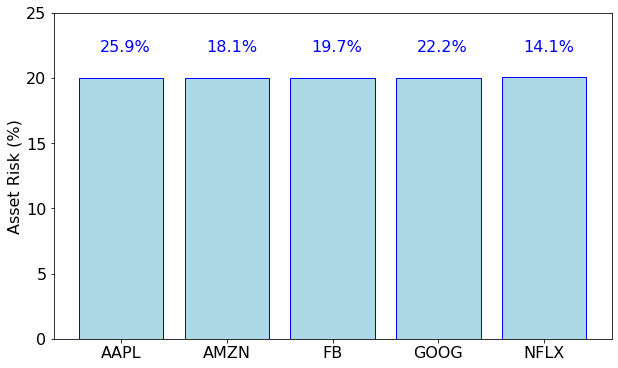
\includegraphics[width=0.7\textwidth]{figures/risk_parity.png}
	\caption{The histogram reports the amount of risk associated to each asset in a risk parity optimization. The label over each bar show the weight of the corresponding asset in the portfolio.}
	\label{fig:risk_parity}
\end{figure}

\subsection{Risk Budget Allocation}\label{risk-budget-allocation}

The same technique can be used if we would like to calculate a portfolio
with risk budget allocation. If we consider the previous equation:

\[ \sigma _{i}=\cfrac{\sigma_p}{N} \]

where we set the risk contribution fraction to every asset to \(1/N\);
now we can simply replace \(1/N\) with the desired fraction (\(f_i\))
for each asset:

\[ \sigma _{i}=f_i \cdot \sigma_p \]
so that the relation to minimise becomes:

\[ \underset{w}{\arg \min } \sum _{i=1}^{N}\left[w_{i}-{\frac {f_i \cdot \sigma_p^{2}}{(\Sigma \mathbf{w})_{i}}}\right]^{2} \]

Translating it to \texttt{python} we get:

    \begin{tcolorbox}[breakable, size=fbox, boxrule=1pt, pad at break*=1mm,colback=cellbackground, colframe=cellborder]
\begin{Verbatim}[commandchars=\\\{\}]
\PY{k}{def} \PY{n+nf}{objective3}\PY{p}{(}\PY{n}{weights}\PY{p}{,} \PY{n}{target\PYZus{}risk}\PY{p}{,} \PY{n}{annual\PYZus{}covariance}\PY{p}{)}\PY{p}{:}
    \PY{n}{variance} \PY{o}{=} \PY{n}{np}\PY{o}{.}\PY{n}{dot}\PY{p}{(}\PY{n}{weights}\PY{o}{.}\PY{n}{T}\PY{p}{,} \PY{n}{np}\PY{o}{.}\PY{n}{dot}\PY{p}{(}\PY{n}{annual\PYZus{}covariance}\PY{p}{,} \PY{n}{weights}\PY{p}{)}\PY{p}{)}
    \PY{n+nb}{sum} \PY{o}{=} \PY{l+m+mi}{0}
    \PY{n}{N} \PY{o}{=} \PY{n+nb}{len}\PY{p}{(}\PY{n}{weights}\PY{p}{)}
    \PY{k}{for} \PY{n}{i} \PY{o+ow}{in} \PY{n+nb}{range}\PY{p}{(}\PY{n}{N}\PY{p}{)}\PY{p}{:}
        \PY{n+nb}{sum} \PY{o}{+}\PY{o}{=} \PY{p}{(}\PY{n}{weights}\PY{p}{[}\PY{n}{i}\PY{p}{]} \PY{o}{\PYZhy{}} \PY{p}{(}\PY{p}{(}\PY{n}{target\PYZus{}risk}\PY{p}{[}\PY{n}{i}\PY{p}{]}\PY{o}{*}\PY{n}{variance}\PY{p}{)}\PY{o}{/}\PY{p}{(}\PY{n}{np}\PY{o}{.}\PY{n}{dot}\PY{p}{(}\PY{n}{annual\PYZus{}covariance}\PY{p}{,} \PY{n}{weights}\PY{p}{)}\PY{p}{[}\PY{n}{i}\PY{p}{]}\PY{p}{)}\PY{p}{)}\PY{p}{)}\PY{o}{*}\PY{o}{*}\PY{l+m+mi}{2}
        
    \PY{k}{return} \PY{n+nb}{sum}

\PY{n}{f\PYZus{}i} \PY{o}{=} \PY{p}{[}\PY{l+m+mf}{0.3}\PY{p}{,} \PY{l+m+mf}{0.2}\PY{p}{,} \PY{l+m+mf}{0.2}\PY{p}{,} \PY{l+m+mf}{0.15}\PY{p}{,} \PY{l+m+mf}{0.15}\PY{p}{]}
\PY{n}{numAssets} \PY{o}{=} \PY{l+m+mi}{5}
\PY{n}{args} \PY{o}{=} \PY{p}{(}\PY{n}{f\PYZus{}i}\PY{p}{,} \PY{n}{annual\PYZus{}covariance}\PY{p}{)}

\PY{n}{constraints} \PY{o}{=} \PY{p}{(}\PY{p}{\PYZob{}}\PY{l+s+s1}{\PYZsq{}}\PY{l+s+s1}{type}\PY{l+s+s1}{\PYZsq{}}\PY{p}{:} \PY{l+s+s1}{\PYZsq{}}\PY{l+s+s1}{eq}\PY{l+s+s1}{\PYZsq{}}\PY{p}{,} \PY{l+s+s1}{\PYZsq{}}\PY{l+s+s1}{fun}\PY{l+s+s1}{\PYZsq{}}\PY{p}{:} \PY{n}{sumWeights}\PY{p}{\PYZcb{}}\PY{p}{)}
\PY{n}{bounds} \PY{o}{=} \PY{n+nb}{tuple}\PY{p}{(}\PY{p}{(}\PY{l+m+mi}{0}\PY{p}{,} \PY{l+m+mi}{1}\PY{p}{)} \PY{k}{for} \PY{n}{asset} \PY{o+ow}{in} \PY{n+nb}{range}\PY{p}{(}\PY{n}{numAssets}\PY{p}{)}\PY{p}{)}

\PY{n}{opts} \PY{o}{=} \PY{n}{optimize}\PY{o}{.}\PY{n}{minimize}\PY{p}{(}\PY{n}{objective3}\PY{p}{,} \PY{n}{np}\PY{o}{.}\PY{n}{ones}\PY{p}{(}\PY{n}{numAssets}\PY{p}{)} \PY{o}{/} \PY{n+nb}{float}\PY{p}{(}\PY{n}{numAssets}\PY{p}{)}\PY{p}{,} \PY{n}{args}\PY{o}{=}\PY{n}{args}\PY{p}{,}
                         \PY{n}{bounds}\PY{o}{=}\PY{n}{bounds}\PY{p}{,} \PY{n}{constraints}\PY{o}{=}\PY{n}{constraints}\PY{p}{)}
\PY{n+nb}{print} \PY{p}{(}\PY{n}{opts}\PY{p}{)}  

\PY{n}{sigma\PYZus{}i} \PY{o}{=} \PY{p}{[}\PY{p}{]}
\PY{k}{for} \PY{n}{i} \PY{o+ow}{in} \PY{n+nb}{range}\PY{p}{(}\PY{n}{numAssets}\PY{p}{)}\PY{p}{:}
    \PY{n}{std} \PY{o}{=} \PY{n}{np}\PY{o}{.}\PY{n}{sqrt}\PY{p}{(}\PY{n}{np}\PY{o}{.}\PY{n}{dot}\PY{p}{(}\PY{n}{opts}\PY{o}{.}\PY{n}{x}\PY{o}{.}\PY{n}{T}\PY{p}{,} \PY{n}{np}\PY{o}{.}\PY{n}{dot}\PY{p}{(}\PY{n}{annual\PYZus{}covariance}\PY{p}{,} \PY{n}{opts}\PY{o}{.}\PY{n}{x}\PY{p}{)}\PY{p}{)}\PY{p}{)}
    \PY{n}{a} \PY{o}{=} \PY{n}{opts}\PY{o}{.}\PY{n}{x}\PY{p}{[}\PY{n}{i}\PY{p}{]}\PY{o}{*}\PY{n}{np}\PY{o}{.}\PY{n}{dot}\PY{p}{(}\PY{n}{annual\PYZus{}covariance}\PY{p}{,} \PY{n}{opts}\PY{o}{.}\PY{n}{x}\PY{p}{)}\PY{p}{[}\PY{n}{i}\PY{p}{]}
    \PY{n}{sigma\PYZus{}i}\PY{o}{.}\PY{n}{append}\PY{p}{(}\PY{n}{a}\PY{o}{/}\PY{n}{std}\PY{p}{)}

\PY{k}{for} \PY{n}{i} \PY{o+ow}{in} \PY{n+nb}{range}\PY{p}{(}\PY{n}{numAssets}\PY{p}{)}\PY{p}{:}
    \PY{n+nb}{print} \PY{p}{(}\PY{l+s+s2}{\PYZdq{}}\PY{l+s+s2}{Risk contribution for asset }\PY{l+s+si}{\PYZob{}\PYZcb{}}\PY{l+s+s2}{: }\PY{l+s+si}{\PYZob{}:.1f\PYZcb{}}\PY{l+s+s2}{\PYZdq{}}\PY{o}{.}\PY{n}{format}\PY{p}{(}\PY{n}{i}\PY{p}{,} \PY{n}{sigma\PYZus{}i}\PY{p}{[}\PY{n}{i}\PY{p}{]}\PY{o}{/}\PY{n+nb}{sum}\PY{p}{(}\PY{n}{sigma\PYZus{}i}\PY{p}{)}\PY{o}{*}\PY{l+m+mi}{100}\PY{p}{)}\PY{p}{)}

     fun: 3.985449091312236e-07
     jac: array([-0.00090474,  0.00038776,  0.0009308 , -0.00032641,  0.0011355
])
 message: 'Optimization terminated successfully.'
    nfev: 45
     nit: 6
    njev: 6
  status: 0
 success: True
       x: array([0.35019494, 0.17972679, 0.18831561, 0.16913951, 0.11262315])
Risk contribution for asset 0: 30.0
Risk contribution for asset 1: 20.0
Risk contribution for asset 2: 20.0
Risk contribution for asset 3: 15.0
Risk contribution for asset 4: 15.0
    \end{Verbatim}
\end{tcolorbox}
Figure~\ref{risk_allocation} shows the amount of risk associated to each asset and their weights within the portfolio. Indeed for each stock we have allocated the desired amount of risk.

\begin{figure}[htb]
	\centering
	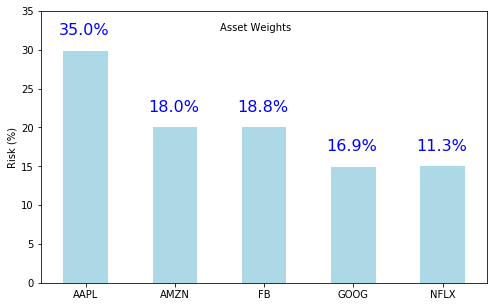
\includegraphics[width=0.7\textwidth]{figures/risk_allocation.png}
	\caption{The histogram reports the amount of risk associated to each asset in a risk allocation optimization. The label over each bar show the weight of the corresponding asset in the portfolio.}
	\label{fig:risk_allocation}
\end{figure}



\section{Maximum Diversification Portfolio}\label{maximum-diversification-portfolio}

In addition to minimum variance, and risk parity/budgeting, maximum diversification is also another well known risk based asset allocation technique.

Diversification is a common topic in portfolio construction. Rather than serving as the sole, quantifiable objective, it is most often either pursued in tandem with another objective, such as return maximization, or pursued simply by including more asset classes or adding constraints based on intuition.

But it does not have to be this way; diversification can be pursued explicitly as the sole objective in portfolio construction.

In a 2008 paper, the diversification ratio $D$ of a portfolio has been defined as:

\[
D=\cfrac{\mathbf{w^T}\boldsymbol{\sigma}}{\sqrt {\mathbf{w^T}\Sigma \mathbf{w}}} 
\]
where $\boldsymbol{\sigma}$ is the vector of volatilities and $\Sigma$ is the covariance matrix. The term in the denominator is the volatility of the portfolio and the term in the numerator is the weighted average volatility of the assets. More diversification within a portfolio decreases the denominator and leads to a higher diversification ratio.

Let's try to construct a portfolio that maximize this ratio.
\begin{tcolorbox}[breakable, size=fbox, boxrule=1pt, pad at break*=1mm,colback=cellbackground, colframe=cellborder]
\begin{Verbatim}[commandchars=\\\{\}]
\PY{k}{def} \PY{n+nf}{calc\PYZus{}diversification\PYZus{}ratio}\PY{p}{(}\PY{n}{w}\PY{p}{)}\PY{p}{:}
\PY{c+c1}{\PYZsh{} average weighted vol}
\PY{n}{w\PYZus{}vol} \PY{o}{=} \PY{n}{np}\PY{o}{.}\PY{n}{dot}\PY{p}{(}\PY{n}{np}\PY{o}{.}\PY{n}{sqrt}\PY{p}{(}\PY{n}{np}\PY{o}{.}\PY{n}{diag}\PY{p}{(}\PY{n}{covariance}\PY{p}{)}\PY{p}{)}\PY{p}{,} \PY{n}{w}\PY{o}{.}\PY{n}{T}\PY{p}{)}
\PY{c+c1}{\PYZsh{} portfolio vol}
\PY{n}{port\PYZus{}vol} \PY{o}{=} \PY{n}{np}\PY{o}{.}\PY{n}{sqrt}\PY{p}{(}\PY{n}{np}\PY{o}{.}\PY{n}{dot}\PY{p}{(}\PY{n}{w}\PY{o}{.}\PY{n}{T}\PY{p}{,} \PY{n}{np}\PY{o}{.}\PY{n}{dot}\PY{p}{(}\PY{n}{covariance}\PY{p}{,} \PY{n}{w}\PY{p}{)}\PY{p}{)}\PY{p}{)}
\PY{n}{diversification\PYZus{}ratio} \PY{o}{=} \PY{n}{w\PYZus{}vol}\PY{o}{/}\PY{n}{port\PYZus{}vol}
\PY{c+c1}{\PYZsh{} return negative for minimization problem (maximize = minimize \PYZhy{})}
\PY{k}{return} \PY{o}{\PYZhy{}}\PY{n}{diversification\PYZus{}ratio}
		
\PY{c+c1}{\PYZsh{} long only: long only constraint}
\PY{n}{bnd} \PY{o}{=} \PY{n+nb}{tuple}\PY{p}{(}\PY{p}{(}\PY{l+m+mi}{0}\PY{p}{,} \PY{l+m+mi}{1}\PY{p}{)} \PY{k}{for} \PY{n}{asset} \PY{o+ow}{in} \PY{n+nb}{range}\PY{p}{(}\PY{n}{numAssets}\PY{p}{)}\PY{p}{)}
\PY{n}{cons} \PY{o}{=} \PY{p}{(}\PY{p}{\PYZob{}}\PY{l+s+s1}{\PYZsq{}}\PY{l+s+s1}{type}\PY{l+s+s1}{\PYZsq{}}\PY{p}{:} \PY{l+s+s1}{\PYZsq{}}\PY{l+s+s1}{eq}\PY{l+s+s1}{\PYZsq{}}\PY{p}{,} \PY{l+s+s1}{\PYZsq{}}\PY{l+s+s1}{fun}\PY{l+s+s1}{\PYZsq{}}\PY{p}{:} \PY{n}{sumWeights}\PY{p}{\PYZcb{}}\PY{p}{,}\PY{p}{)}
\PY{c+c1}{\PYZsh{}if long\PYZus{}only: \PYZsh{} add in long only constraint}
\PY{c+c1}{\PYZsh{}cons = cons + (\PYZob{}\PYZsq{}type\PYZsq{}: \PYZsq{}ineq\PYZsq{}, \PYZsq{}fun\PYZsq{}:  long\PYZus{}only\PYZus{}constraint\PYZcb{},)}
\PY{n}{opts} \PY{o}{=} \PY{n}{optimize}\PY{o}{.}\PY{n}{minimize}\PY{p}{(}\PY{n}{calc\PYZus{}diversification\PYZus{}ratio}\PY{p}{,} \PY{n}{np}\PY{o}{.}\PY{n}{ones}\PY{p}{(}\PY{n}{numAssets}\PY{p}{)} \PY{o}{/} \PY{n+nb}{float}\PY{p}{(}\PY{n}{numAssets}\PY{p}{)}
\PY{p}{,} \PY{n}{bounds}\PY{o}{=}\PY{n}{bnd}\PY{p}{,} 
\PY{n}{method}\PY{o}{=}\PY{l+s+s1}{\PYZsq{}}\PY{l+s+s1}{SLSQP}\PY{l+s+s1}{\PYZsq{}}\PY{p}{,} \PY{n}{constraints}\PY{o}{=}\PY{n}{cons}\PY{p}{)}
\PY{n+nb}{print} \PY{p}{(}\PY{n}{opts}\PY{p}{)}
\PY{n}{ret} \PY{o}{=} \PY{n}{np}\PY{o}{.}\PY{n}{sum}\PY{p}{(}\PY{n}{annual\PYZus{}expected}\PY{o}{*}\PY{n}{opts}\PY{o}{.}\PY{n}{x}\PY{p}{)}
\PY{n}{vol} \PY{o}{=} \PY{n}{np}\PY{o}{.}\PY{n}{sqrt}\PY{p}{(}\PY{n}{np}\PY{o}{.}\PY{n}{dot}\PY{p}{(}\PY{n}{opts}\PY{o}{.}\PY{n}{x}\PY{o}{.}\PY{n}{T}\PY{p}{,} \PY{n}{np}\PY{o}{.}\PY{n}{dot}\PY{p}{(}\PY{n}{annual\PYZus{}covariance}\PY{p}{,} \PY{n}{opts}\PY{o}{.}\PY{n}{x}\PY{p}{)}\PY{p}{)}\PY{p}{)} 
\PY{n+nb}{print} \PY{p}{(}\PY{l+s+s2}{\PYZdq{}}\PY{l+s+s2}{Diversification: }\PY{l+s+s2}{\PYZdq{}}\PY{p}{,} \PY{o}{\PYZhy{}}\PY{n}{opts}\PY{o}{.}\PY{n}{fun}\PY{p}{)}

fun: -1.3820226890251621
jac: array([-1.87858939e-04,  1.40175223e-04, -3.96057963e-04, -7.59512186e-05, 6.11126423e-04])
message: 'Optimization terminated successfully.'
nfev: 42
nit: 6
njev: 6
status: 0
success: True
x: array([0.35727486, 0.17943996, 0.17225915, 0.09847119, 0.19255483])

Diversification:  1.3820226890251621
\end{Verbatim}
\end{tcolorbox}

Figure~\ref{fig:max_div} shows how the maximum diversified portfolio compare to the efficient frontier.

\begin{figure}[htb]
	\centering
	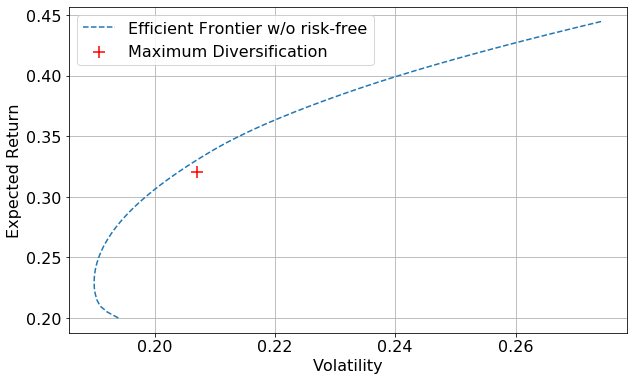
\includegraphics[width=0.7\textwidth]{figures/max_div.png}
	\caption{Portfolio constructed with the maximum diversification technique shown in the return/variance plane.}
	\label{fig:max_div}
\end{figure}
